
\documentclass[11pt]{article}
 
\usepackage[margin=1in]{geometry} 
\usepackage{amsmath,amsthm,amssymb}
\usepackage{graphicx} 
\usepackage{blkarray}
\usepackage{amsmath}




\newcommand{\N}{\mathbb{N}}
\newcommand{\Z}{\mathbb{Z}}
 
\newenvironment{problem}[2][Problem]{\begin{trivlist}
\item[\hskip \labelsep {\bfseries #1}\hskip \labelsep {\bfseries #2.}]}{\end{trivlist}}
\newenvironment{lemma}[2][Lemma]{\begin{trivlist}
\item[\hskip \labelsep {\bfseries #1}\hskip \labelsep {\bfseries #2.}]}{\end{trivlist}}
\newenvironment{exercise}[2][Exercise]{\begin{trivlist}
\item[\hskip \labelsep {\bfseries #1}\hskip \labelsep {\bfseries #2.}]}{\end{trivlist}}

\newenvironment{question}[2][Question]{\begin{trivlist}
\item[\hskip \labelsep {\bfseries #1}\hskip \labelsep {\bfseries #2.}]}{\end{trivlist}}
\newenvironment{corollary}[2][Corollary]{\begin{trivlist}
\item[\hskip \labelsep {\bfseries #1}\hskip \labelsep {\bfseries #2.}]}{\end{trivlist}}

\usepackage{indentfirst}
\linespread{1.2}     % 调整间距
\setlength{\parindent}{0pt}

\begin{document}

 
% --------------------------------------------------------------
%                         Start here
% --------------------------------------------------------------
 
\title{Homework 8 DS-GA 1002 }%replace X with the appropriate number
\author{Yuhao Zhao\\ %replace with your name
Yz3085} %if necessary, replace with your course title
 
\maketitle
\begin{problem}{1}
\end{problem}
a) The condition mean minimize the mean square error.\\
 Therefore, $g_{MSE}(Y) = E(X|Y) $.\\
 for $y\in [-3,-1], x =-1$ with probability 1,$g_{MSE}(Y) = 1$\\ 
 for $y\in [1,3], x =1$ with probability 1,$g_{MSE}(Y) = -1$\\
 for $y\in [-1,1], x =1$ with p = 0.5 and x =-1 with p=0.5,$g_{MSE}(Y) = 0.5-0.5 = 0$\\
 
 
 b) $P(X \neq g_{MSE}) = P(X = 1)P(g_{MSE} \neq 1|X=1) + P(X = 0)P(g_{MSE} \neq 0|X=0)$\\
 = $P(y\in[-1,1])\times 1 = P(x=1)P(y\in[-1,1]|x=1)+P(x=-1)P(y\in[-1,1]|x=-1) = \frac{1}{4}+\frac{1}{4} = \frac{1}{2}$ \\
 
 c) MAP estimation minimize the probability of error\\
 $g_{error} = g_{MAP}(y) =\underset{x \in \{1, -1\}} {\mathrm{Argmin}} ~ P_{X|Y}(X|Y) =\underset{x \in \{1, -1\}} {\mathrm{Argmin}} ~ \frac{f_{Y|X}(y|X=x) P(X = x)}{f_y(y)}  $\\
 $Y|X \sim Uniform(X-2,X+2)$\\
 Therefore, $g_{MAP}(y)  =1$ if $ \frac{1}{4}\times I(y\in[-1,3])\times \frac{1}{2}> \frac{1}{4}\times I(y\in[-3,1])\times \frac{1}{2}$\\
 This means, $g_{MAP}(y) = 1$ if $y\in [1,3]$ and $g_{MAP}(y) = 0$  if  $y\in [-3,-1]$\\
 For $y \in [-1,1]$ we choose arbitrarily.\\
 
 $P(x\neq g_{MAP}(y)) =P(X = 1)P(g_{MAP} \neq 1|X=1) + P(X = 0)P(g_{MAP} \neq 0|X=0) $\\
 = $\frac{1}{2} \times P(y\in [-1,1]|X=1)\times \frac{1}{2} + \frac{1}{2} \times P(y\in [-1,1]|X=0)\times \frac{1}{2}$\\
 = $\frac{1}{2}\frac{1}{2}\frac{1}{2}+\frac{1}{2}\frac{1}{2}\frac{1}{2} = \frac{1}{4}$\\
 
 d)$MSE(g_{error}) = E((x - g_{MAP}(y))^2) = E(x^2) + E(g_{MPA}^2) -2E(xg_{MAP})$\\
 = 1 + 1 -$2E(xE(g_{MAP}(y|x))) = 2 - 2(\frac{1}{2}(1\times \frac{1}{2})+\frac{1}{2}(-1\times -\frac{1}{2})) = 1$ 
 
  
 
 \begin{problem}{2}
 \end{problem}
a) $g_{MAP}(w) =\underset{R \in \{1, 0\}} {\mathrm{Argmin}} ~ P_{R|W}(R|W)  = \underset{R \in \{1, 0\}} {\mathrm{Argmin}} ~ \frac{P_{W|R}(W|R)P(R)}{P(W)}$\\
$g_{MAP}(w)  = 1 $ if $ \frac{P_{W|R=1}(W|R=1)P(R=1)}{P(W)}>\frac{P_{W|R=0}(W|R=0)P(R=0)}{P(W)}$ and $g_{MAP}(w)  = 0$ otherwise\\
for $w =1, 0.7\times 0.2 < 0.3\times 0.8, g_{MAP}(w)  = 0$ \\
for $w =0, 0.3\times 0.2 < 0.7\times 0.8, g_{MAP}(w)  = 0$ \\
Therefore, $g_{MAP} = 0$ whatever w is. This means the prediction given the forecast is not rain whatever the forecast is.\\

b) It's more reasonable to assume H and W are independent given R. H and W are not mutually independent, because rain or not should be dependent on the humidity, the weather forecast should be dependent on humidity. \\

c)  $H|R=1 \sim uinf(0.5,0.7), H|R=0 \sim unif(0.1,0.6)$\\
$g_{MAP}(w) =\underset{R \in \{1, 0\}} {\mathrm{Argmin}} ~ P_{R|W,H}(R|W,H)  = \underset{R \in \{1, 0\}} {\mathrm{Argmin}} ~\frac{f_{W,H|R}\times P_R(R)}{f_{W,H}}=\underset{R \in \{1, 0\}} {\mathrm{Argmin}} ~\frac{P_{W|R}\times f_{H|R}\times P_R(R)}{f_{W,H}} $ \\by conditional Independence.\\
$g_{MAP}(w)  = 1 $ if $ 0.2 P_{W|R=1} \times \frac{1}{0.2} I(H\in[0.5,0.7]) >0.8f_{W|R=0} \times \frac{1}{0.5}I(H \in [0.1,0.6])$ and $g_{MAP}(w)  = 0$ otherwise\\

H= 0.65,W=0,  \quad $0.2 \times 0.3\times 5 > 0.8 \times0.7\times 2\time 0$\\
$g_{MAP} =1$\\

d) H=0.55, w = 1, \quad $0.2\times  0.7 \times 5 > 0.8\times 0.3 \times 2$\\
$g_{MAP} =1$\\

e)$P(R \neq g_{MAP}) = P(R = 0)P(g_{MAP}=1|R=0) +P(R = 1)P(g_{MAP}=0|R=1)$\\
The case that the estimation could be wrong is w=1,H$\in[0.1,0.5]$ and w =0, H$\in [0.5,0.6]$\\
$P(R \neq g_{MAP}) = 0.8\times P(w=1|R=0)\times P(H\in[0.1,0.5]|R=0))+ 0.2 \times P(w=0|R=0\times P(H\in[0.6,0.7]|R=1)) = 0.8 \times 0.3 \times 0.2 + 0.2 \times 0.3\times 0.5 = 0.048+0.03 = 0.078$\\

\begin{problem}{3}
\end{problem}
a)$g_{MAP}(S,C) = \underset{H \in \{1, 0\}} {\mathrm{Argmin}} ~ P_{H|S,C}(H|S,C) =  \underset{H \in \{1, 0\}} {\mathrm{Argmin}} ~\frac{P_{S,C|H}\times P_H(H)}{P_{S,C}}= \underset{H \in \{1, 0\}} {\mathrm{Argmin}} ~\frac{P_{S|H}\times P_{C|H}\times P_H(H)}{P_{S,C}} $\\ by conditional independence\\
$g_{MAP} = 1 $  if $\frac{P_{S|H=1}\times P_{C|H=1}\times P_H(H=1)}{P_{S,C}} > \frac{P_{S|H=0}\times P_{C|H=0}\times P_H(H=0)}{P_{S,C}}$\\
$g_{MAP} = 0 $ otherwise.\\

b)\begin{verbatim}
P_S_H0 >>> array([ 0.42735043,  0.57264957])
P_S_H1 >>> array([ 0.14851485,  0.85148515])
P_C_H0 >>> array([ 0.09401709,  0.24786325,  0.4017094 ,  0.25641026])
P_C_H1 >>> array([ 0.03960396,  0.06930693,  0.16831683,  0.72277228])

Probability of error 0.18
\end{verbatim}

c)$g_{MAP}(S,C,X) = \underset{H \in \{1, 0\}} {\mathrm{Argmin}} ~ P_{H|S,C}(H|S,C,X) =  \underset{H \in \{1, 0\}} {\mathrm{Argmin}} ~\frac{P_{S,C,X|H}\times P_H(H)}{P_{S,C,X}}=\\ \underset{H \in \{1, 0\}} {\mathrm{Argmin}} ~\frac{P_{S|H}\times P_{C|H}\times f(X|H)\times P_H(H)}{P_{S,C}} $ by conditional independence\\

$g_{MAP} = 1 $  if $\frac{P_{S|H=1}\times P_{C|H=1}\times f(X|H=1)\times P_H(H=1)}{P_{S,C}} > \frac{P_{S|H=0}\times P_{C|H=0}\times f(X|H=0)\times P_H(H=0)}{P_{S,C}}$\\
$g_{MAP} = 0$ otherwise\\

d)\begin{verbatim}
mean_X_H >>> array([ 245.57264957,  254.02970297])
std_X_H >>> array([ 46.52070879,  45.01890812])
\end{verbatim}

 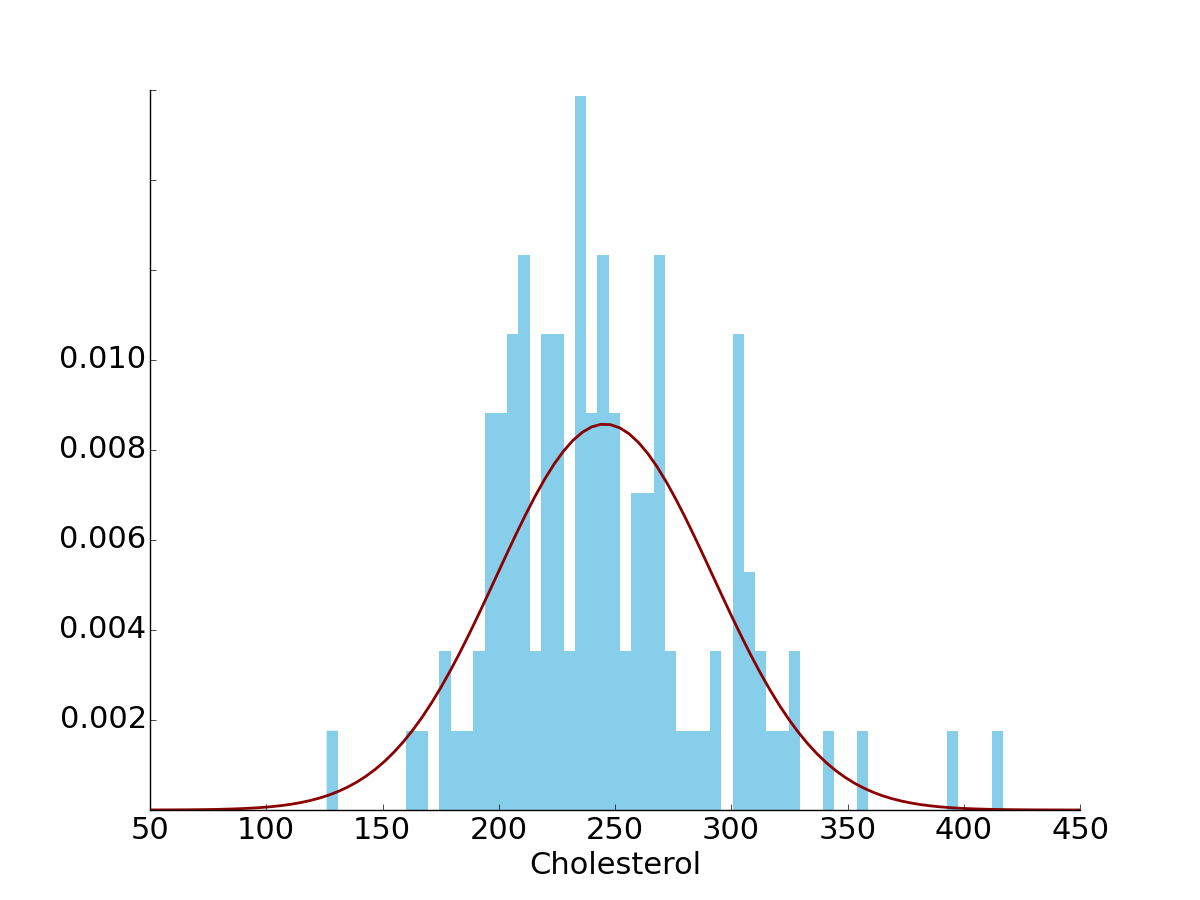
\includegraphics[height =2.5in]{245}
  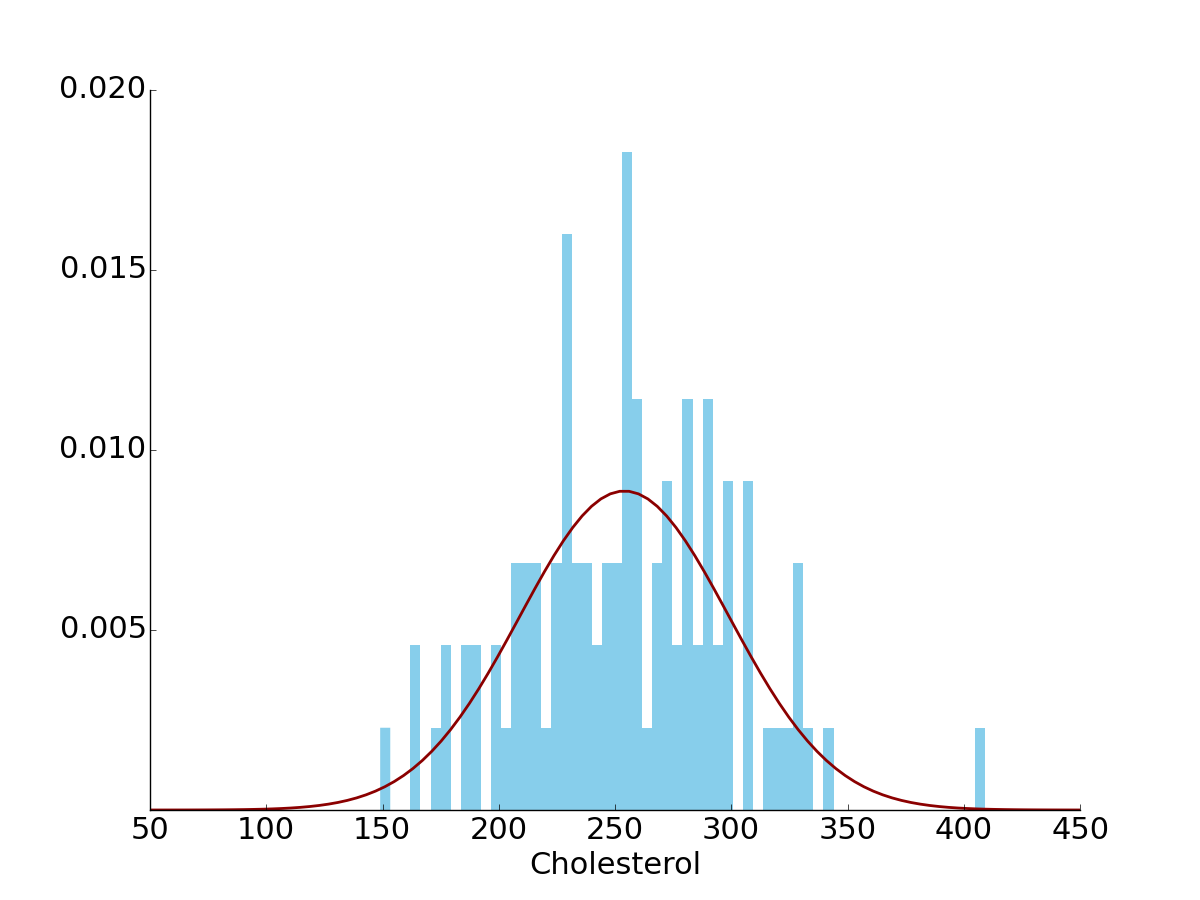
\includegraphics[height =2.5in]{254}
  \begin{verbatim}
             Cholesterol with H=0                      Cholesterol with H=1
  \end{verbatim}

e)Incorporating with the cholesterol data, we have a new probability of error 0.14. \\

We can't trust this result, because the Cholesterol data doesn't seems to be perfectly normally distributed from the histograms. What's more, if we conduct a pairwise t-test to cholesterol level with H=0 and H=1, we have a p-value 0.177. This means we don't have enough evidence to conclude that  people with different H have difference in cholesterol. Therefore it's not reasonable to include the cholesterol into the Bayesian model.  \\

f) 





\end{document}